\documentclass{article}

% Language setting
% Replace `english' with e.g. `spanish' to change the document language
\usepackage[english]{babel}

% Set page size and margins
% Replace `letterpaper' with `a4paper' for UK/EU standard size \usepackage[letterpaper,top=2cm,bottom=2cm,left=3cm,right=3cm,marginparwidth=1.75cm]{geometry}
% Useful packages
\usepackage{amsmath}
\usepackage{graphicx}
\usepackage{multirow}
\usepackage{booktabs}
\usepackage[colorlinks=true, allcolors=blue]{hyperref}

\title{Video Query Processing with Text}
\author{Sinclair Hudson}

\begin{document}
\maketitle

\begin{abstract}
      This work explores different ways to leverage large language models (LLMs) to convert video into textual descriptions, and then further answer queries about the video using the textual descriptions.
      VideoDescriptor?
      VidDesc?
\end{abstract}

\section{Introduction}

We propose a video understanding pipeline using LLMs that can be used to...
% TODO hmmm
Simultaneously, the performance of language models has surged in recent years, largely thanks to the predictable scaling of transformer-based models.
This work proposes a general pipeline for accomplishing video understanding tasks using multimodal LLMs, by converting visual information into text and then completing the analog task in the text domain.

\section{Related Work}

\subsection{Video Understanding}

Video understanding is difficult for many reasons.
The data is very high-dimensional, and yet semantically sparse; most frames and pixels are redundant when analysing the video for content.
% TODO mention video compression here, and how it's really successful because of structural biases in video.
Additionally, video-data is extremely time-consuming to annotate.
As such, very few video datasets exist, and are often much smaller than analogous image datasets \cite{imagenet} \cite{COCO}.
Nevertheless, videos are ubiquitous in digital life, and so the research domain of video understanding is active and diverse.

CLIP4Clip is a method that aims to extend the ideas of CLIP \cite{clip} to the video domain \cite{clip4clip}.
It generally follows a bi-encoder structure, in which the video and text are encoded using separate transformers \cite{transformer}.
The video is split into different patches spatially, and each patch is encoded using a linear layer into an embedding vector, and then processed by the video encoder transformer.
Then, both representations are fed into a similarity calculator module.
The system is trained end-to-end with contrastive loss, as in CLIP \cite{clip}.

X-CLIP takes a similar approach to CLIP4Clip, using contrastive pre-training between videos and text to learn associations between video and textual descriptions \cite{xclip}.
However, X-CLIP goes further and models more fine-grained associations between video and text.
For a given video-caption pair, the video is encoded frame-by-frame are then passed into a temporal encoder, producing both a vector for each frame and a vector for the entire video.
Likewise, the caption is encoded using a transformer, producing both a vector for the entire caption and a vector for each word.
X-CLIP explicitly models caption-video, caption-frame, word-video, and word-frame relationships, and uses these associations to learn very detailed representations of the video and text.
These representations, along with task-specific fine-tuning, allow X-CLIP to perform very well on text-to-video and video-to-text retrieval tasks.

InternVideo is a recent attempt at a "foundation model" for video, being able to complete numerous downstream tasks.
The authors train InternVideo with a combination of multimodal constrastive learning (as in CLIP \cite{clip}), as well as masked video reconstruction, inspired by VideoMAE \cite{videomae}.
The InternVideo video encoder is pretrained on a large dataset of internet videos and movies, allowing it to learn very semantically rich representations of videos.
With additional fine-tuning on specific tasks, InternVideo achieves state-of-the-art performance on multiple tasks including Action Understanding, Video-Language Alignment, and Video Open Understanding \cite{internvideo}.
Pipelines that use Internvideo are often combined with TODO in order to bridge the modality gap between video and text. Note that InternVideo is \textit{not} a large language model.

\subsection{Large Language Models for Vision}

Some other 

Flamingo

LLaVA \cite{llava} is a large language model trained on a combination of text and video data, build upon TODO. 
It is build upon the Vicuana language model \cite{vicuana}, and incorporates the visual encoder of CLIP \cite{clip} to encode images into embeddings that the language model can take as input.
It is fine-tuned end-to-end on instructional image-text data.
It has proven to be exceptionally strong at visual question-answering tasks, ... TODO

\subsection{Large Language Models for Video}

Most related to this work are attempts to leverage large language models for video understanding tasks.

VideoChat \cite{videochat} focuses on an understanding of video that is amenable to multiple-round video question answering.
The proposed approach is similar to that taken in VideoChat-Text; the pipeline first seeks to convert the video into a textual description, and then uses that textual description for downstream tasks involving the video.

Video-ChatGPT \cite{videochatgpt} is a method similar to the proposed pipeline, in that it adapts LLaVA to process video intead of images.
In their approach, the video is embedded both frame-wise and spatial-patch-wise, allowing for the model to learn both temporal and spatial features.
% TODO this doesn't make sense
This video embedding module is trained, while the down-stream LLM and video encoder remain frozen. As such, this can be seen as a parameter-efficient fine-tuning approach to adapt LLaVA to video.




\subsection{Video-Text datasets}
MSR-VTT (Microsoft Research Video to Text) is a flagship video understanding dataset \cite{msr-vtt}.
This dataset can be used for multiple tasks, including Video Question Answering, Video Retrieval, and Video Captioning.
The dataset contains 10,000 videos, largely sourced from the internet (TODO verify).
For the video retrieval task, 1000 queries are used for testing, each specifying exactly one video as the correct answer \cite{jsfusion}.
The videos in the video retrieval split are 12 seconds long on average, see \ref{fig:length_histogram} for a histogram of video lengths.

\begin{figure}
      \centering
      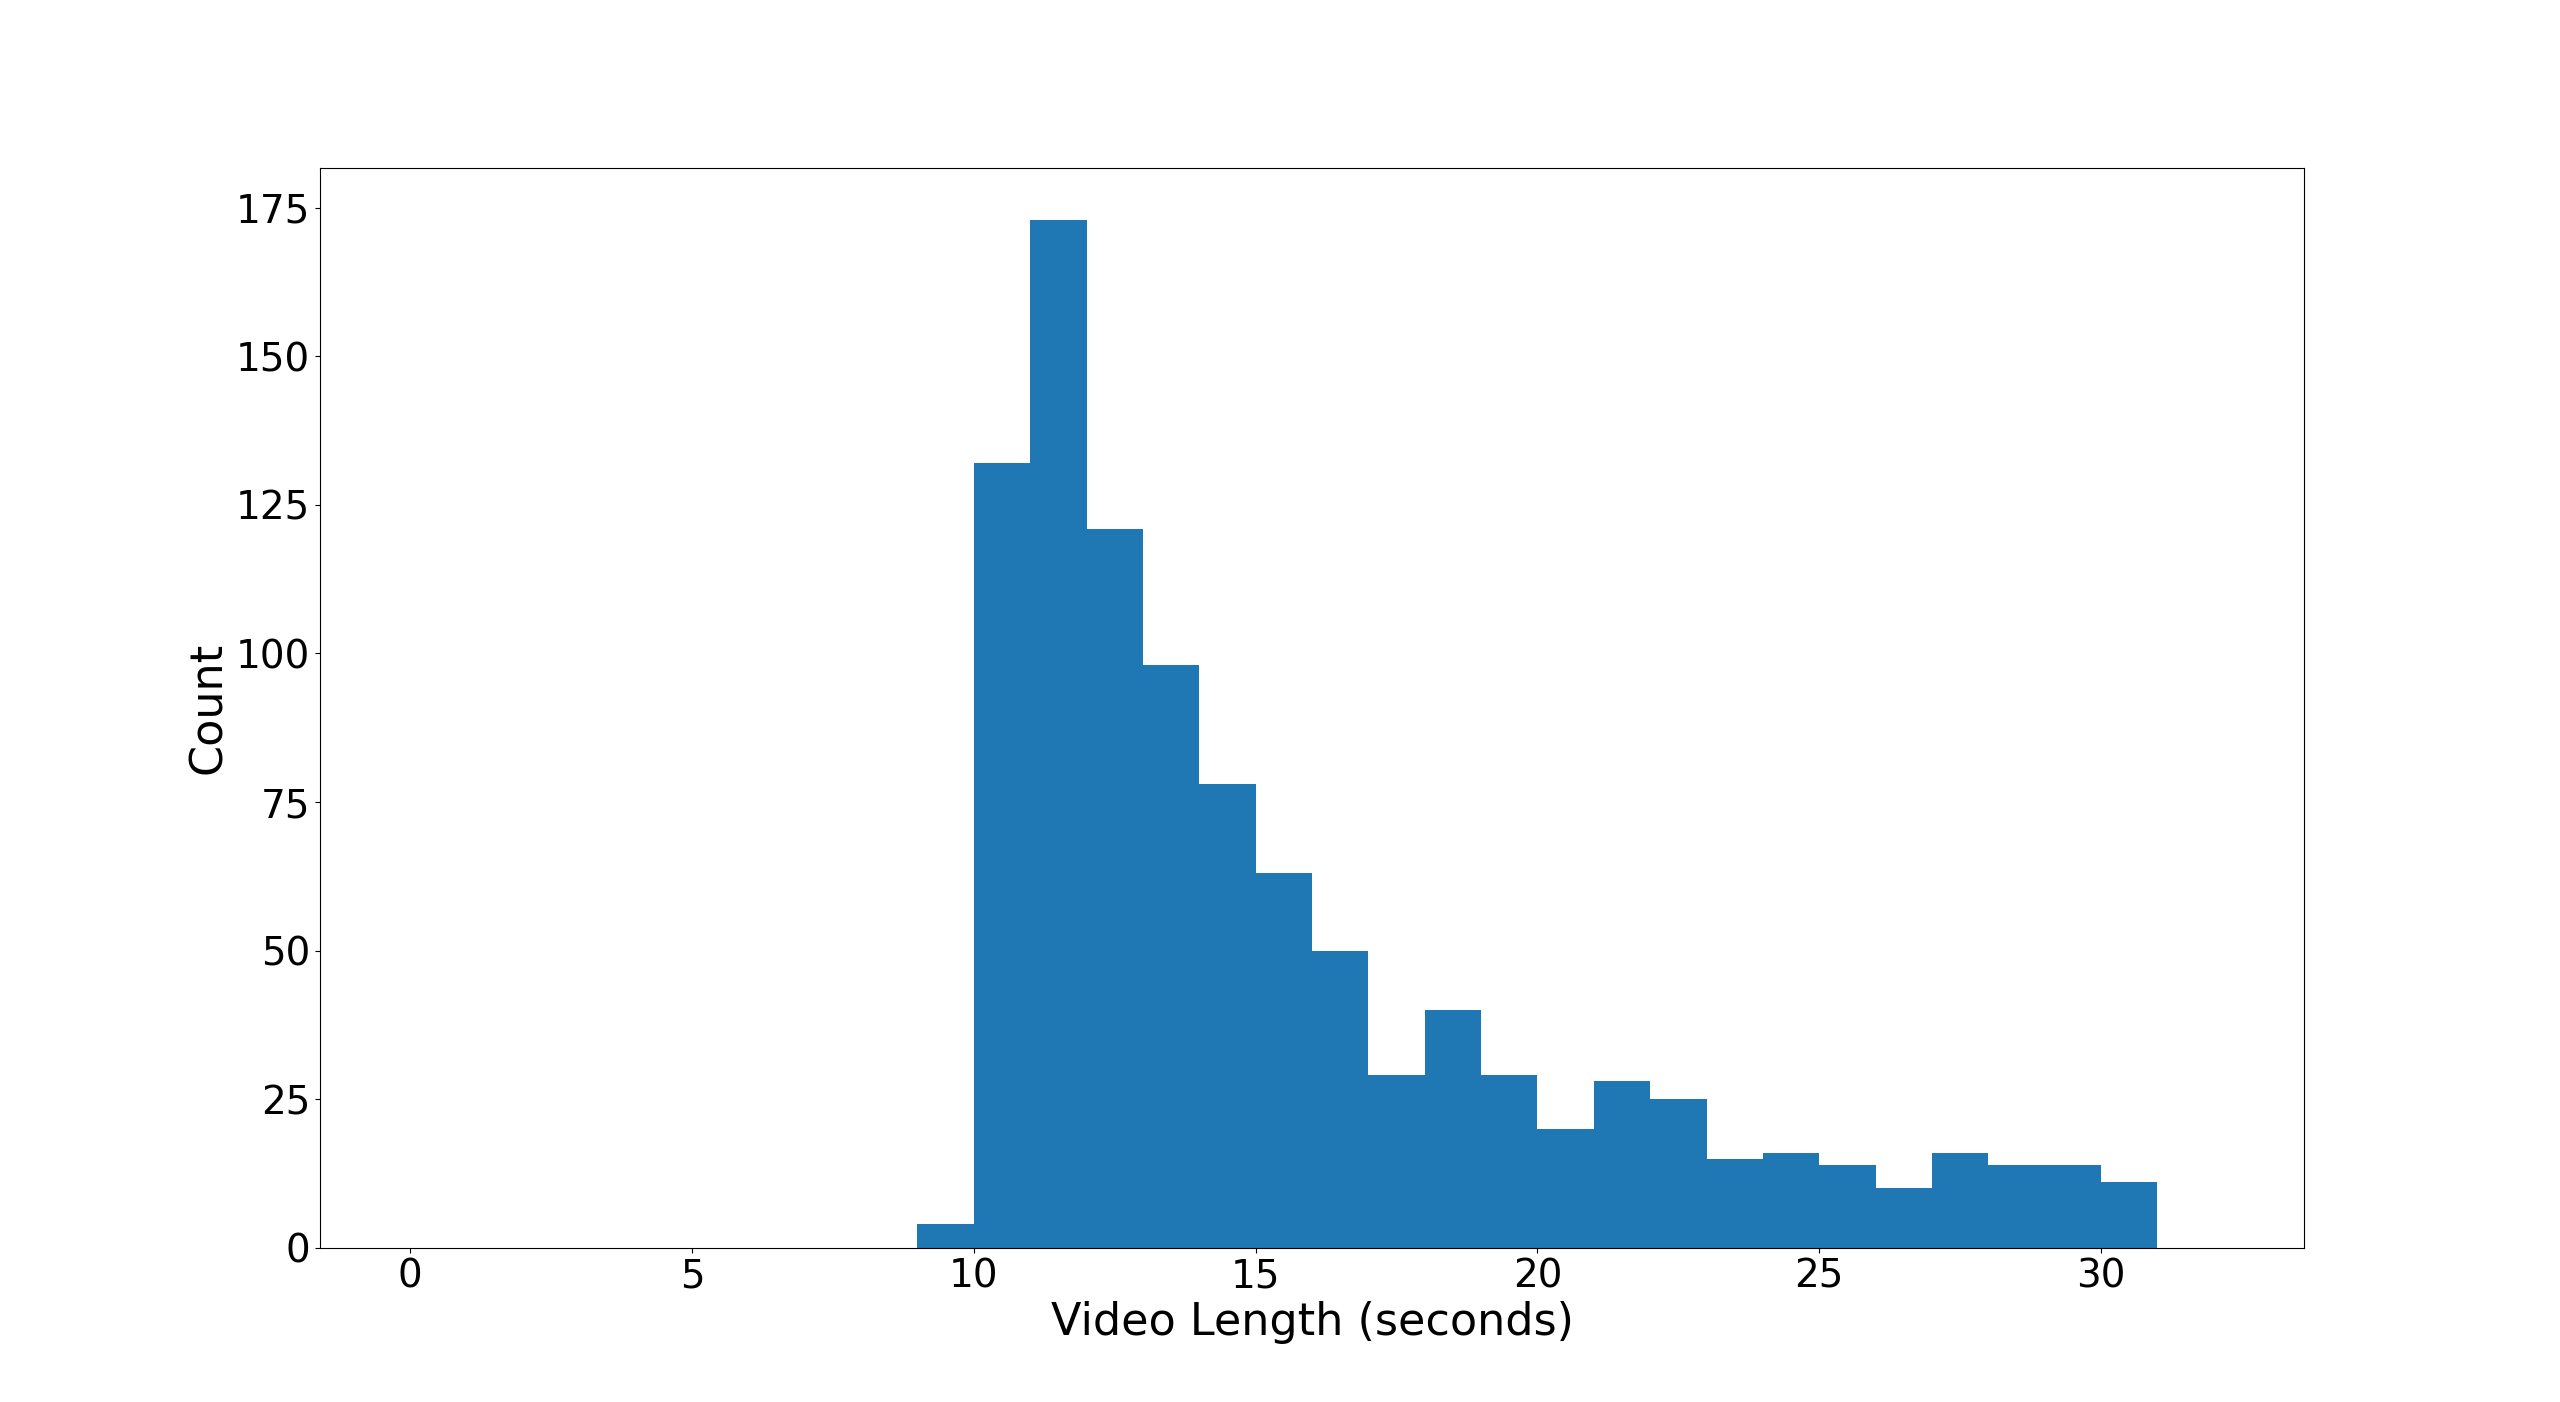
\includegraphics[width=\textwidth]{figures/msr-vtt-length-histogram.png}
      \caption{Length of videos in the MSR-VTT retrieval data split.}
      \label{fig:length_histogram}
\end{figure}

\section{Method}

\begin{figure}
      \centering
      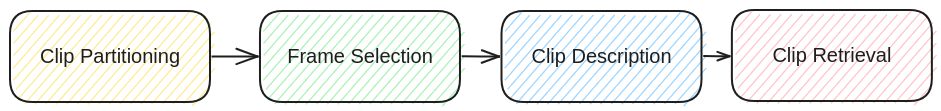
\includegraphics[width=0.8\textwidth]{figures/pipeline.png}
      \caption{High level block diagram of the proposed video understanding pipeline.}
      \label{fig:pipeline}
\end{figure}

The proposed pipeline is designed in such a way to be general to different video understanding tasks, with each of the 4 major steps allowing for multiple methods, or being optional for some tasks.
For the purposes of this work, a "clip" is a small segment of a video that is a few seconds long, 
and is highly cohesive in what it depicts. For example, in a movie, a clip might be a single shot.
At a high level, the pipeline for video understanding using LLMs is as follows:
\begin{enumerate}
      \item Partition the video into individual clips (optional)
      \item From each clip, select a small subset of frames to represent the clip
      \item Using the selected frames, generate a textual description of the clip using an LLM.
      \item Using the textual description, answer queries about the video, or retrieve clips.
\end{enumerate}

For brevity, these steps will be referred to as "Clip partitioning", "Frame selection", "Clip description", and "Clip Retrieval" respectively.
The two most applicable tasks for this pipeline are video retrieval and video summarization.
In video retrieval, given a query, the goal is to retrieve the video in a video dataset that best matches the query.
In visual video summarization, the goal is to edit a video down to a shorter length, containing only clips relevant to a given query.
Prior works often treat the video as-is and do not pre-process it much.



\section{Clip Partitioning}

Videos can contain a lot of different clips, which may or may not be related.
The input for clip partitioning is the whole video, and the output is a list of breaks (frame numbers) between clips.
The difficult aspect of clip partitioning is to efficiently find the boundaries between clips.
A two-hour video at 24 frames per second contains 172,800 frames, and so processing each one is computationally expensive.
\subsection{Uniform partitioning}
The simplest approach to clip partitioning is to simply partition the video into equal-sized clips, without regard for the content of the video.
This approach is simple, but the resulting clips are not necessarily cohesive, since clips could contain multiple scenes and shots.
\subsection{Coarse-to-fine clip partitioning}
Starts by computing the L1 distance between frames 1 second apart.
If the the distance is above a certain threshold, then a clip break is likely in this second.
Thus, the 1-second segment is evaluated frame by frame, and if the distance between two frames is above a threshold, then a clip break is identified.

\begin{figure}
      \centering
      \includegraphics[width=0.8\textwidth]{figures/TODO.png}
      \caption{Frames one before and one after a clip break, determined by the coarse-to-fine clip partitioning strategy. The movie being partitioned is TODO}
      \label{fig:optical_flow}
\end{figure}


\section{Frame Selection}

Even within a single clip, there are a lot of frames, most of which are very similar to their neighbours.
To make the pipeline efficient, it's critical to select the subset of the most semantically relevant frames.
LLMs can only effectively interpret one image at a time (todo verify).
The input to frame selection is a clip (small length of video) and the output is a list of frames selected for further processing.

Earlier works simply sample randomly \cite{TODO} or sample uniformly, at a course framerate such as 1 frame per second \cite{clip4clip}.

This work explores 3 different frame selection strategies:
greedy L1 selection, stratified sampling, and TODO.

\subsection{Stratified Sampling}
To get a potentially more diverse set of frames, the first, last and middle frames are selected.
We call this sampling method \verb|3-strat|. We also explore \verb|5-strat|, which selects the first, last, and 3 evenly spaced frames in between.

\subsection{Stratified Triplet Sampling}
It's possible that the stratified sampling method above is too coarse, and that a single frames at multiple points in the clip is not enough to capture the clip's content.
For this reason, this work also explores stratified triplet sampling, where at each of the 3 points in the clip, 3 frames are selected across 1 second.
The motivation for this method is that the 3 frames in a single second will show what is changing in the scene.
each triplet is fed in as a single input into the LLM, which can take multiple images as input.
As a result, there is only one textual description per triplet in this sampling method.

\subsection{Greedy L1 Selection}
Greedy L1 selection initially selects the first frame of a clip. Then, it selects an additional clip if the L1 distance between the new frame and the previously selected frame is greater than some threshold (for example).
The L1 distance is normalized by the number of pixels in the image, so that the threshold is independent of the video resolution.
In the MSR-VTT dataset, most videos are quite short (TODO graph for this), and often only contain a single shot.
As such, when using Greedy L1 selection, a substantial number of videos only have the first frame selected (with L1 threshold 180).
The idea for selction based on L1 is to skip frames that are visually similar to the previously selected frame.
The selection strategy is greedy; the first frame is always selected, and then frames are considered in order, only selected if the frame differs from the previously selected frame by a certain L1 distance.
More formally

% TODO maybe just write an algorithm block for this? It's not difficult
\begin{equation}
      c < \frac{|I_{p} - I_{c}|}{W \times H \times C}
\end{equation}
where $c$ is a pre-defined threshold, $I_{p}$ is the previously selected frame, $I_{c}$ is the current frame, and $W$, $H$, $C$ are the width, height, and channels of the frames, respectively.

\begin{figure}
      \centering
      \includegraphics[width=0.8\textwidth]{figures/L1_frame_selection.png}
      \caption{Number of frames selected per video in the MSR-VTT dataset retrieval split, for different thresholds.}
      \label{fig:optical_flow}
\end{figure}

L1 was chosen over L2 because L2 is very sensitive to large changes in a few pixels; L1 gives a better sense of the overall change in the image.

\section{Prompting Strategies}

The LLM used in testing this pipeline is LLava \cite{llava}.
LLaVA is selected because it is free and open source, and can be run on a single consumer GPU, making it amenable to experimentation.

Beam search, multiple prompts with a temperature.
Two prompts are tried in this work, one of which is is dubbed "concise" (C), while the other is "verbose" (V).
The concise prompt is ""
The verbose prompt is "Please describe the objects in this image. Be as descriptive as possible."
For getting a textual description of a single image, the prompt used is "Please describe the objects in this image. Be as descriptive as possible.".
LLM performance can be sensitive to prompts.

The input to the LLM is a prompt and (potentially) multiple frames, and the output is a text caption.
In all cases, we limit the length of the caption to 512 words, to bound the amount of computation required per frame.

\section{Retrieval}

The last aspect of 

Because LLMs have described the content of the videos, the retrieval task is reduced to that of text retrieval, which is well-studied.
In this work, we explore two retrieval strategies: BM25 and Bi-Encoder, using OpenAI embeddings.
BM25 is a highly performant sparse retriever, relying on term frequencies TODO.

\subsection{Bi-Encoder Retrieval}

This approach is heavily inspired by DPR \cite{dpr}, but uses the same encoder for both documents and queries, and uses L2 distance as a similarity metric instead of the dot product.
In that way, it's similar to the Bi-Encoder strategy used in the BLINK zero-shot entity linker \cite{blink}.
Specifically, the OpenAI model used to generate embedding vectors is \verb|text-embedding-ada-002|, which outputs 1536-dimensional vectors.
The KNN is performed using the FAISS library \cite{faiss}, and all clip descriptions are embedded and stored in an index beforehand, making querying for nearest neighbours very fast.

\section{Results}

\subsection{Video Retrieval}

\begin{table}[htbp]
  \centering
  \begin{tabular}{lcccc}
    \toprule
    \textbf{Benchmark} & \multicolumn{3}{c}{\textbf{MSR-VTT}} \\
    \cmidrule(lr){2-4}
                       prompt & \textbf{R@1} & \textbf{R@5} & \textbf{FT} & \textbf{Size} \\
    \midrule
    \multirow{2}{*}{CLIP4Clip} & 0.85 & 0.88 & 0.90 \\
    & (0.02) & (0.01) & (0.03) \\
    \midrule
    \multirow{2}{*}{XCLIP} & 0.78 & 0.82 & 0.85 \\
    & (0.03) & (0.02) & (0.01) \\
    \midrule
    \multirow{2}{*}{InternVideo} & 0.92 & 0.89 & 0.91 \\
    & (0.01) & (0.02) & (0.01) \\
    \bottomrule
    % TODO add my own results.
  \end{tabular}
  \label{tab:model_comparison}
  \caption{Performance Comparison of Models on Different Benchmarks. B}
\end{table}

Note that due to computational constraints, only the 1000 videos in the MSR-VTT retrieval split were indexed, while in related works the entire dataset of 10,000 videos are indexed.
As such, direct comparisons between the recall values between this work and related works should not be made.
The retrieval task for the proposed pipeline is much easier, since it is retrieving from a dataset one tenth the size.
Also note that this pipeline functions zero-shot, while all other models have been finetuned for text-to-video retrieval on MSR-VTT.

\subsection{Qualitative Results on Video Summarization}
For video summarization, the task is to select a subset of clips from a video relevant to the query.
Sports games are desireable to summarize because they are long, with a few well-defined interesting events (goals, fouls, etc.).
To test this method, we will full sports games from YouTube.
In this full soccer game, 7 goals are scored, 4 by France and 3 by Argentina.

\begin{table}[htbp]
  \centering
  \begin{tabular}{lccccc}
    \toprule
    \textbf{Query} & \multicolumn{3}{c}{\textbf{Soccer}} & \multicolumn{3}{c}{\textbf{Hockey}}\\
    \cmidrule(lr){2-4}
    & \textbf{Recall} & Length \\
    \midrule
    \multirow{2}{*}{Goals Scored by team France, in dark blue jerseys.} & 0.85 & 0.88 & 0.90 & HR, HL, \\
    & (0.02) & (0.01) & (0.03) \\
    \midrule
    \multirow{2}{*}{Goals scored by team Argentina, in light blue and white jerseys.} & 0.78 & 0.82 & 0.85 \\
    & (0.03) & (0.02) & (0.01) \\
    \midrule
    \multirow{2}{*}{Goals scored} & 0.92 & 0.89 & 0.91 \\
    & (0.01) & (0.02) & (0.01) \\
    \bottomrule
  \end{tabular}
  \label{tab:video_summarization}
  \caption{Performance Comparison of Models on Different Benchmarks}
\end{table}

\section{Discussion}

Interestingly, the experiments that use "triple" frames don't perform notably better than the experiments that use single frames in video retrieval.
This seems to suggest that either the additional frames are redundant, or that LLaVA is not good at incorporating information from multiple images in a single generation step.
This is similar to the findings in CLIP4clip, where the authors find that processing frames in batches as 3D tensors doesn't improve performance over frame-by-frame processing \cite{clip4clip}.

The authors of VideoChat note that their similar VideoChat-Text pipeline struggled to understand "intricate temporal reasoning and causal inference".

\section{Future work}

Expanding methodologies to other datasets is critical to fully examine the generalization capability of these pipelines.
Additionally, this pipeline currently is very slow, requiring many forward passes of a large language model for every frame, and multiple frames for every clip.
Future work could investigate further minimizing the number of frames processed, and prompting techniques to generate very dense captions, with a lot of information content in few tokens.
Finally, while this work focused on the visual features of video, audio is also often attached to video, and thus could be used to further improve the performance of the pipeline.
Related work such as VideoLLaMA has shown that audio can provide a small boost to performance \cite{videollama}.
Incoporating audio would be particularly important for understanding videos that have an emphasis on dialogue, such as movies.
The current pipeline is experimental in nature, and has not been optimized for runtime performance.
With additional engineering effort, the performance of the video processing and text processing elements of the pipeline could both be greatly improved.
Future work could also further investigate the influence of prompts and different LLMs on the performance of the pipeline.

\section{Conclusion}

\bibliographystyle{alpha}
\bibliography{biblio}

\end{document}
